%----------------------------------------------------------------------------------------
%	PACKETS AND CONFIGURATION
%----------------------------------------------------------------------------------------

\documentclass[11pt]{beamer}
\setbeamercovered{transparent}

\usepackage{title}  		% Title settings for the presentation
\usepackage{parskip}    	% Paragraph indent & skip
\usepackage{xcolor}     	% More colors
\usepackage{enumitem}		% Better lists
\usepackage{graphicx}  		% 'graphics' package interface
\usepackage{listings}   	% Code sections formatting}
%\usepackage{pdftexcmds}
%\usepackage{minted}
%\usepackage[utf8]{inputenc}
%\usepackage[T1]{fontenc}
%\usepackage{pythontex}
\usepackage{verbatim}
\usepackage{amsmath}

% Custom colors
\definecolor{AnnotationPurple}{RGB}{103, 13, 173}
\definecolor{CommentGreen}{RGB}{29, 204, 49}

% Python code formatting
% Use it by creating an environment like \begin{lstlisting}[style=Python] ... \end{lstlisting}
% Since annotations aren't tagged as keywords I have inserted a manual delimiter for them,
% it works as follows: \@@AnnotationText@@/
\lstdefinestyle{Python}{
    language = Python,
    basicstyle = \footnotesize\ttfamily,
    commentstyle = \textcolor{CommentGreen},
    stringstyle = \textcolor{orange},
    showstringspaces = false,
    keywordstyle = \textcolor{blue},
    moredelim = [is][\textcolor{AnnotationPurple}]{\\@}{@@\/},   % Annotations
    numberstyle = \scriptsize\ttfamily\textcolor{gray},
    numbers = left,
    frame = single,
    frameround = tttt,
    framexleftmargin = 10pt,
    framexrightmargin = 0pt
}

% PowerPoint-style Presentation
%\centering

% HELPER PACKAGES (TODO: REMOVE IN FINAL) %
\usepackage{todonotes}
\presetkeys{todonotes}{inline}{}
\usepackage{blindtext}
% HELPER PACKAGES (TODO: REMOVE IN FINAL) %

\usetheme{Antibes} % THEME

%----------------------------------------------------------------------------------------
%	DOCUMENT
%----------------------------------------------------------------------------------------

\begin{document}

% TITLE
\frame{\titlepage}

% Table of Contents
\begin{frame}{Presentation Outline}
\begin{tiny}
    \vspace*{-1em}
    \tableofcontents[hideallsubsections]
\end{tiny}
\end{frame}

% Section overview
\AtBeginSection[]
{
\begin{frame}{}
    \tableofcontents[sections={\thesection}]
\end{frame}
}

% Introduction ------------------------------------------------------------

\section{Introduction}

% ----------------------------------------

% ----------------------------------------

\subsection{Assignment}

% ----------------------------------------

\begin{frame}

\frametitle{Project Scope}
\framesubtitle{Assignment}

The focus of this project is to optimize the budget allocated for the \textbf{advertisement campaigns} of 5 different items in order to maximize the profit of an \textit{e-commerce website} that sells products to the public.

Each page has a \textbf{primary product} and some \textbf{secondary products}, each user that lands on a page has a possibility to buy the primary prodcut and/or proceed to one of the secondaries with a given probability, the process repeats.

\end{frame}


% ----------------------------------------

\begin{frame}

\frametitle{General hypoteses}

The main general hypoteses that were given to us are:
\begin{itemize}[label={-}]
    \item For every \textit{primary product}, the \textit{secondary products} to display and their order is fixed.
    \item The price of every product is fixed and it is equal to the margin.
    \item By clicking on a specific ad, the user lands on the corresponding \textit{primary product}.
\end{itemize}

\end{frame}

% ----------------------------------------

\subsection{Technical Approach}

% ----------------------------------------

\begin{frame}

\frametitle{Learner interface}
\framesubtitle{Description}

In order for our project to have a more general outline, we decided to model a \textbf{generic learner interface} to standardize how our agents should be expected to behave while learning the budget distribution for a set of subcampaigns in a specific scenario defined by the environment.

In particular, each learner is characterized by the \textit{learn} and \textit{predict} actions.
Every different type of learner will also receive a customized set of information filtered by the \textit{masked environment} (in line with each project step) and potentially employs different algorithms to learn and predict the various budgets.

\end{frame}

% ----------------------------------------

\begin{frame}[fragile]

\frametitle{Learner interface}
\framesubtitle{Code}

%Arguments: interactions: the interactions of the users which led to the given reward reward: the reward obtained from the environment based on the prediction given, needed for the tuning of internal properties done by the learner
%prediction: array containing the previous budget evaluation of the learner
%
%Arguments: data: up-to-date, complete or incomplete environment information that is used by the learner in order to make the inference
%Returns: a tuple containing a list of values (corresponding to the budgets inferred given the knowledge obtained by the learner until now) and a list of features (referring to which particular customers were the budgets aimed for, if None, the budgets apply to all the customers)

\begin{lstlisting}[style=Python, basicstyle=\tiny, numbers=none, framexrightmargin=-20pt]
class Learner(ABC):

  # Updates the learner's properties according to the reward received.
  \@@abstractmethod@@/
  def learn(self, interactions: List[Interaction], reward: float,
            prediction: np.ndarray):
    pass

  # Makes an inference about the values of the budgets for the subcampaigns
  # from the information got over time and the current environment
  \@@abstractmethod@@/
  def predict(self, data: MaskedEnvironmentData) ->
              Tuple[np.ndarray, Optional[List[List[Feature]]]]:
    pass

  # Creates a figure and plots showing the status of learning progress
  \@@abstractmethod@@/
  def show_progress(self, fig: plt.Figure):
    pass

\end{lstlisting}

\end{frame}

% ----------------------------------------

\begin{frame}

\frametitle{Comparing results}

For each different learner, when possible, we will show our results through the comparison of the rewards obtained by each algorithm against the rewards achieved (in the same enviroment setting) from the \textbf{Clairvoyant learner} and the Stupid learner.
This, aside from theoretical formulations, will help us to define \textbf{upper bounds} and \textbf{lower bounds} for different solutions.

In particular, the \textbf{Clairvoyant learner} makes its "prediction" with full knowledge of the problem while the stupid learner always subdivides \textit{equally} the budget between products.

\end{frame}

% ----------------------------------------

\begin{frame}

\frametitle{Comparing results}
\framesubtitle{Clairvoyant learner}

\todo{Our implementation for the clairvoyant learner - also mention non determinism and blueprint system}

\end{frame}

% ----------------------------------------

\begin{frame}

\frametitle{Comparing results}
\framesubtitle{Regret}

\todo{General regret formulation: see slides 1-05 and 1-06}

\end{frame}

% ----------------------------------------

\begin{frame}

\frametitle{Gaussian processes}

\todo{GP description: see slides 3-05}

\end{frame}

% ----------------------------------------

\begin{frame}

\frametitle{UCB1 formulation}
\framesubtitle{Outline}

In the \textbf{UCB1} algorithm, every \textit{arm} is associated with an \textbf{upper confidence bound} which provides an \textit{estimation} of the reward gained by playing that specific arm.

When each arm has been played at least once in order to have a baseline for its reward, at every trial, the arm with the \textbf{highest upper confidence bound} is pulled (\textit{optimism in the face of uncertainty}).
After having collected the realization of the reward for the chosen arm, its \textit{upper confidence bound} is updated accordingly.

The main advantage of combining \textbf{gaussian processes} with \textbf{UCB1} is that, in this way it's possible to take advantage of the \textbf{GP}'s \textit{confidence interval} by modeling it as a \textbf{confidence bound}.

\end{frame}

% ----------------------------------------

\begin{frame}[fragile]

\frametitle{UCB1 formulation}
\framesubtitle{Formalities}

Code snippet that calculates the \textbf{upper bound}:

\begin{lstlisting}[style=Python, basicstyle=\tiny, numbers=none, framexrightmargin=-20pt]
def estimation(self):
  upper_bounds = (self.means + self.confidence * 1.96 * self.sigmas)
                   * self.normalize_factor
  return upper_bounds
\end{lstlisting}

The \textit{theoretical regret} given by this kind of algorithm is bounded by:

\begin{displaymath}
R(UCB1) \le \sum_{a:\mu_a < \mu_a^*} \frac{4log(T)}{\Delta_a} + 8\Delta_a
\end{displaymath}

where $\Delta_a$ is the difference in expected reward between the \\ optimal arm $a^*$ and the arm $a$: $\Delta_a = \mu_a^* - \mu_a$

\end{frame}

% ----------------------------------------

\begin{frame}

\frametitle{TS formulation}
\framesubtitle{Outline}

Some aspects of \textbf{TS} are similar to the \textbf{UCB1} since both are bandit algorithms, the main difference is that in \textbf{TS} every arm is associated to a $prior \beta distribution$.

Every arm has a prior on its \textbf{expected value} based on its mean distribution.
After drawing a sample according to the corresponding prior distribution, the algorithm chooses the arm with the \textbf{best sample}, then, it updates the distribution of the chosen arm according the observed realization.

Both \textbf{Thompson Sampling} (\textbf{TS}) and \textbf{Upper Confidence Bound} (\textbf{UCB}, in particular \textbf{UCB1}), in conjunction with \textbf{Gaussian Processes} are the base algorithms chosen for the learners in our project.

\end{frame}

% ----------------------------------------

\begin{frame}[fragile]

\frametitle{TS formulation}
\framesubtitle{Formalities}

The \textit{theoretical regret} given by this kind of algorithm is bounded by:

\begin{displaymath}
R(TS) \le (1+\epsilon) \sum_{a:\mu_a < \mu_a^*} \frac{\Delta_a(log(T)+log(log(T)))}{K*\Lambda(\mu_a*, \mu_a)} + C (\epsilon, \mu_{a_1} , ... , \mu_{a_{\left|A\right|}})
\end{displaymath}

where $K*\Lambda(mu_a*,mu_a)$ is the \textbf{Kullback-Leibler divergence} and, as before, $\Delta_a$ is defiened as the difference in expected reward between the optimal arm $a^*$ and the arm $a$: $\Delta_a = \mu_a^* - \mu_a$

\end{frame}

% ----------------------------------------


% ----------------------------------------

% Environment and Simulation ----------------------------------------------

\section{Environment and Simulation}

% ----------------------------------------

% ----------------------------------------

\subsection{Overview}

% ----------------------------------------

\begin{frame}

\frametitle{Assumptions}
\framesubtitle{E-commerce website}

For this project, we are required to design an \textbf{Environment} that satisfies various constraints both on the e-commerce site's properties and on the users' behavior; in addition, since most of the tasks were generic, we had to come up with some of our own assumptions.

In particular we want to underline the following assumptions for the e-commerce website:
\begin{itemize}[label={-}]
    \item The website has unlimited stock for the 5 different items.
    \item Actions on the various webpages are \textbf{perfectly observable} by the e-commerce website.
\end{itemize}

\end{frame}

% ----------------------------------------

\begin{frame}

\frametitle{Assumptions}
\framesubtitle{Users}

...and we assume that the users present the following behaviors:
\begin{itemize}[label={-}]
    \item Every day, there is a random number (subject to noise) of potential new users.
    \item The users can activate \textbf{parallel paths} while on the website.
    \item The number of items that a user will buy is a random variable, independent from any other variable; but every user that lands on the page of a product will buy at least 1 unit of it if it's under their \textbf{reservation price}.
    \item The behavior of users can be modelled as a graph where \textit{nodes} represent product pages and \textit{weights} represent the probabilities for a user to click from the primary item of the page to one of the secondaries.
\end{itemize}

\end{frame}

% ----------------------------------------

\subsection{Environment structure}

% ----------------------------------------

\begin{frame}[fragile]

\frametitle{Environment}
\framesubtitle{Structure}

The environment is modelled as a python dataclass containing the following attributes:

\begin{lstlisting}[style=Python, basicstyle=\tiny, numbers=none, framexrightmargin=-20pt]
    # The total budget to subdivide
    total_budget: int

    # Probability of every class to show up. They must add up to 1
    class_ratios: List[float]

    # Features associated to every class
    class_features: List[List]

    # Price of the 5 products
    product_prices: List[float]

    # List of class parameters for each class and product,
    # implemented as list of lists of UserClassParameters.
    # Each class has distinct parameters for every product
    classes_parameters: List[List[UserClassParameters]]
\end{lstlisting}

\end{frame}

% ----------------------------------------

\begin{frame}[fragile]

\frametitle{Environment}
\framesubtitle{Structure}

\begin{lstlisting}[style=Python, basicstyle=\tiny, numbers=none, framexrightmargin=-20pt]
    # Lambda parameter, which is the probability of osserving the
    # next secondary product according to the project's assignment
    lam: float

    # Max number of items a customer can buy of a certain product.
    # The number of bought items is determined randomly with
    # max_items as upper bound
    max_items: int

    # Products graph's matrix. It's a empty matrix, should be
    # initialized with populate_graphs
    graph: np.ndarray

    # List that constains for every i+1 product the secondary i+1
    # products that will be shown in the first and second slot
    next_products: List[Tuple[int, int]]

    # Controls randomness of the environment
    random_noise: float
\end{lstlisting}

\end{frame}

% ----------------------------------------

\begin{frame}

\frametitle{Environment}
\framesubtitle{Masked Environment}

Alongside the \textbf{Environment} we define a \textbf{Masked Environment} with the purpose of \textit{hiding crucial information} to the learners since each type of learner should only have access to a subset of all the information available in the environment dictated by the type of learner.

The masked environment isn't strictly needed in the project since the learners could easily ignore the extra information, however, we wanted to face the problem with an approach aimed towards reusability and extendability and in this case (as in many others down the line) we opted for a more \textbf{generalizable} solution.

\end{frame}

% ----------------------------------------

\begin{frame}

\frametitle{Users}
\framesubtitle{User parameters}

We modelled the $\alpha$-functions, which compute the expected value of interactions on a product given a fixed budget, as \textbf{exponential functions}.

In particular their \textit{upper bound} represents the maximum expected number of interactions possible while the \textit{maximum useful budget} is the amount of budget after which any budget increase would not lead to a ratio increase.

\end{frame}

% ----------------------------------------

\begin{frame}

\frametitle{Users}
\framesubtitle{User classes}

Users are subdivided in classes based on their \textit{2 binary features} for a total of \textit{3 different classes}.

In particular, each user class is defined by its $\alpha$-functions (one for each product plus the one for the non-strategic competitor) which define the probability of landing on a given product page.

Each $\alpha$-function is defined by the values: \textbf{reservation price}, \textbf{upper bound} and \textbf{maximum useful budget}

\end{frame}

% ----------------------------------------

\subsection{Randomness in the Environment}

% ----------------------------------------

\begin{frame}

\frametitle{Randomness in the Environment}
\framesubtitle{Non determinism}

For the sake of representing a real scenario, most of the values that are not known a priori are \textit{randomly generated} and every variable that evolves through time without our direct control has elements of randomness to it (for instance, each day we randomly get the number of active total users in our scenario by using a gaussian distribution with tunable mean and standard deviation).

Even though most of the randomness is tunable and controlled through seeded generators, there are still \textbf{impactful elements of non determinism} (i.e. the Dirichlet distribution) that are not possible to control in any way.

\end{frame}

% ----------------------------------------

\subsection{Simulation}

% ----------------------------------------

\begin{frame}

\frametitle{Daily Simulation}
\framesubtitle{Purpose}

The \textbf{Simulation} class is the main engine that brings together \textit{learners} and \textit{environment} by making them interact with each other while offering an interface to customize the execution.

The basic idea of the simulation is to simulate a real scenario day by day using the environment to generate interactions with the website according to the budgets that the current learner proposed and then, feed the results back to the learner to make it actually learn.

Repeating the simulation execution step for each day until an arbitrary \textbf{time horizon} is reached grants us all the data needed to evaluate the performance of our learner.

\end{frame}

% ----------------------------------------

\begin{frame}

\frametitle{Daily Simulation}
\framesubtitle{Example}

\scriptsize
Simulation runs of two learners in an environment with total\_budget = 400 and population\_mean = 1000

\begin{center}
    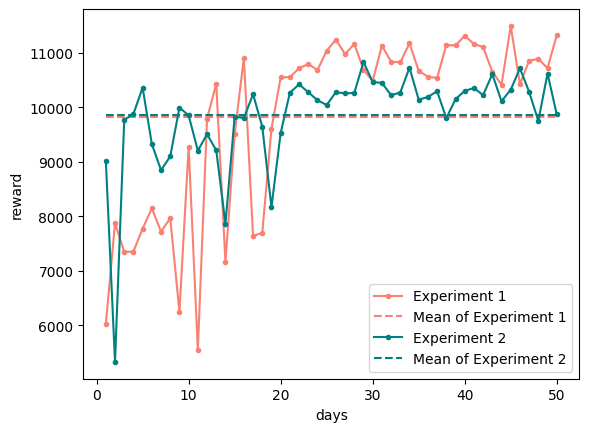
\includegraphics[scale=0.5]{img/Graphs/env_sim/image1.png}
\end{center}


\end{frame}

% ----------------------------------------


% ----------------------------------------

% Optimization Algorithm --------------------------------------------------

\section{Optimization Algorithm}

% ----------------------------------------

% ----------------------------------------

\subsection{General Problem}

% ----------------------------------------

\begin{frame}

\frametitle{Problem formulation}

The purpose of the \textbf{optimization algorithm} is to find the \textit{optimal budget} for each campaign in order to maximize the \textit{profit}, which is defined as the difference between the profits gained from selling products and the advertisement expenses.

Basically, it is a maximization problem subject to an obvious constraint: the sum of the daily budget can't be greater then the overall budget.

The optimization problem can be expressed as follows:
\begin{displaymath}
	F=\max_{\substack{x_i\in B}} \sum_{i=0}^n \alpha_i(x_i)p_i-x_i ~\text{  s.t.  } \sum_{i=0}^n x_i\leq B
\end{displaymath}

\end{frame}

% ----------------------------------------

\subsection{Algorithm}

% ----------------------------------------

\begin{frame}

\frametitle{Code}
\framesubtitle{Functioning}

\vspace*{-1em}

Given a \textbf{budget assignment problem} over the matrix $c$, which is assumed to be divided into $n$ rows (campaigns) and $m$ columns (budget fractions from 0 to $B$ \textit{maximum budget}).

We solve this problem via \textbf{DP} and we start by setting up \textbf{two extra tables} to store the \textit{best values} and their \textit{relative allocations}, then we iterate over each row and column finding the best index for each cell by taking into consideration the sum between the current and the previous row matching budgets; we store the best values and their indexes in the corresponding tables.

The optimal allocation lies at the end of the of the updated table, however, in order to obtain a final allocation which fully utilizes the whole budget we trace back the best values table \textbf{greedily} adding sub-optimal allocations until our budget runs out.

\end{frame}

% ----------------------------------------

\begin{frame}[fragile]

\frametitle{Code}
\framesubtitle{Example}

\begin{lstlisting}[style=Python, basicstyle=\tiny, numbers=none, framexrightmargin=-20pt]
dp = [c[0]]
allocs = [np.arange(m)]

for i in range(1, n):
	next_dp_row = []
	next_alloc_row = []
	for j in range(m):
		prev_row_r = dp[i - 1][j::-1]
		curr_row = c[i][: j + 1]

		row_sum = prev_row_r + curr_row

		# The best index is the index which we should select for
		# the maximum profit, it will be what we store in
		# allocation, and we will also store the value of the
		# row_sum at best_index to dp[i][j]
		best_index = np.argmax(row_sum)

		next_alloc_row.append(best_index)
		next_dp_row.append(row_sum[best_index])

	allocs.append(np.array(next_alloc_row))
	dp.append(np.array(next_dp_row))

dp = np.array(dp)
allocs = np.array(allocs)
# ...
\end{lstlisting}

\end{frame}

% ----------------------------------------

\begin{frame}[fragile]

\frametitle{Code}
\framesubtitle{Example}

\begin{lstlisting}[style=Python, basicstyle=\tiny, numbers=none, framexrightmargin=-20pt]
# ...
best_dp_index = np.argmax(dp[-1])

# As we stored the allocation of what the dp would mean, we now need to
# trace back through the allocs array to create the final allocation
last_alloc = allocs[-1][best_dp_index]

final_allocs = [last_alloc]
remaining_budget = m - last_alloc

for i in range(n - 2, -1, -1):
	# Based on the remaining_budget, we take the max of the remaining
	# possible cumulative values that we have in the dynamic
	# programming table
	sub_dp = dp[i, :remaining_budget]
	sub_best_index = np.argmax(sub_dp) if len(sub_dp) > 0 else 0

	next_alloc = allocs[i][sub_best_index]
	final_allocs.append(next_alloc)

	remaining_budget = remaining_budget - next_alloc

# As we constructed the the final allocation from the back to front,
# we need to reverse it before returning it
return np.array(list(reversed(final_allocs)))
\end{lstlisting}

\end{frame}

% ----------------------------------------


% ----------------------------------------

% Uncertain alpha functions -----------------------------------------------

% ----------------------------------------

\section{Uncertain $\alpha$-functions}

% ----------------------------------------

% ----------------------------------------

\subsection{Contextual hypotesis}

% ----------------------------------------

\begin{frame}

\frametitle{Scenario}

We now assume that the binary features of the users cannot be observed and therefore data is considered as \textbf{aggregated}.

Since the features of the users are \textbf{not observable}, the $\alpha$ functions' shape for each class is unknown.

As a result, in our scenario the learner receives all the interactions minus the parameters of the $\alpha$ functions.

\end{frame}

% ----------------------------------------

\subsection{Algorithm}

% ----------------------------------------

\begin{frame}

\frametitle{Solving the problem}

By gathering the aggregated reward for each product we are able to utilize those coarse rewards to generate feedbacks for our \textbf{MABs} and therefore train them on the aggregated interactions for each day.

In particular we exploit \textbf{Gaussian Processes} in conjunction with \textbf{MAB} algorithms such as \textbf{Thompson Sampling} and \textbf{UCB1} to exploit the continuity between the different arms.

We instantiate a \textbf{GP-MAB} for each subcampaign and each \textbf{MAB} will have \texttt{n\_budget\_steps} number of arms.

\end{frame}

% ----------------------------------------

\begin{frame}

\frametitle{Algorithms outline}
\framesubtitle{GP TS}

\textbf{GPTS} is a variant of \textbf{TS} implemented using \textbf{Gaussian Processes}:

\begin{itemize}[label={$\circ$}]
	\item For each day $t$, we gather a sample from each arm $a$:
		\begin{displaymath}
			\tilde{\theta_a} \leftarrow \text{ Sample} \left( \mathbb{P}(\mu_a = \theta_a) \right)
		\end{displaymath}
	\item Play arm $a_t$ defined as:
		\begin{displaymath}
			a_t \leftarrow arg\max_{a \in A} \left\{ \tilde{\theta_a} \right\}
		\end{displaymath}
	\item Update the \textbf{Gaussian Process} with the reward obtained.
\end{itemize}

\end{frame}

% ----------------------------------------

\begin{frame}[fragile]

\frametitle{Algorithms outline}
\framesubtitle{GP UCB1}

\textbf{GPUCB1} is a variant of \textbf{UCB1} that takes advantage of the \textbf{Gaussian Processes} confidence interval and models it as the confidence bound; apart from the arm choice, the learning process is equal to \textbf{GPTS}.

\begin{displaymath}
	a_t \leftarrow arg\max_{a \in A} \left\{ \mu_{t-1} + \delta \sigma_{t-1} \right\}
\end{displaymath}

Code snippet that calculates the \textbf{upper bound}:

\begin{lstlisting}[style=Python, basicstyle=\tiny, numbers=none, xrightmargin=15px]
def estimation(self):
	upper_bounds = (self.means + self.confidence * 1.96 * self.sigmas)
			* self.normalize_factor
	return upper_bounds
\end{lstlisting}

\end{frame}

% ----------------------------------------

\subsection{Results}

% ----------------------------------------

\begin{frame}[plain]

\frametitle{Single run reward and regret}
\framesubtitle{Thompson Sampling and UCB}

\begin{center}
	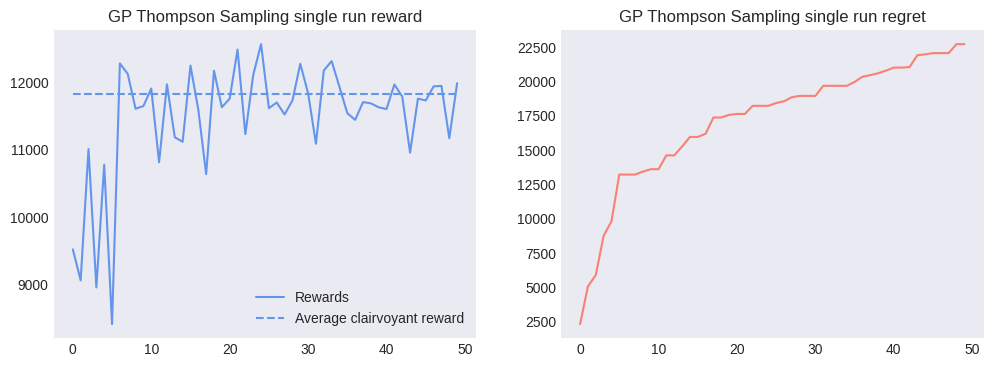
\includegraphics[scale=0.4]{img/Graphs/uncertain_alpha/image1.png}
	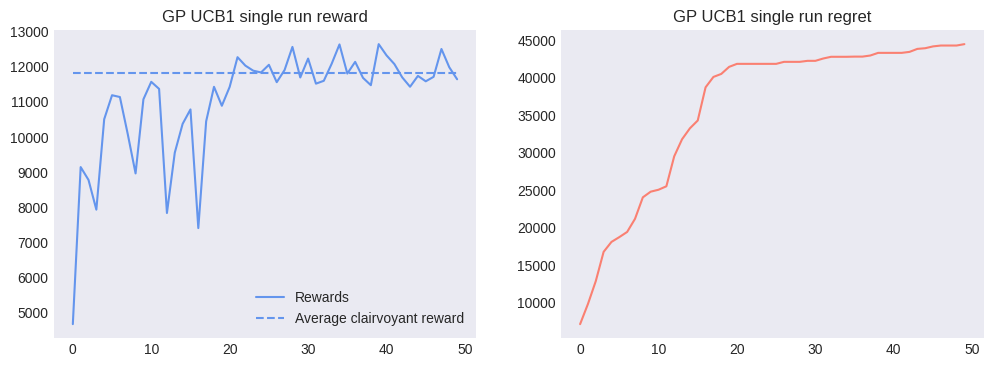
\includegraphics[scale=0.4]{img/Graphs/uncertain_alpha/image2.png}
\end{center}

\end{frame}

% ----------------------------------------

\begin{frame}[plain]

\frametitle{Regret comparison}
\framesubtitle{Thompson Sampling and UCB}

\begin{center}
	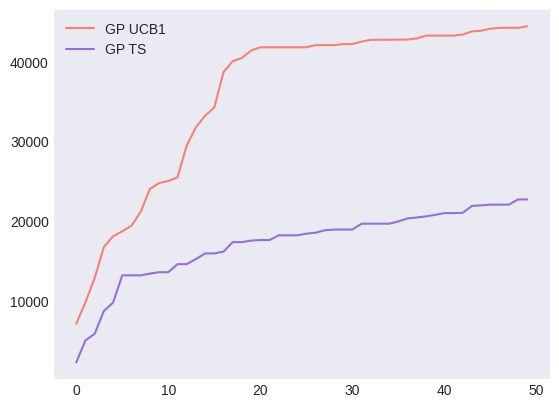
\includegraphics[scale=0.5]{img/Graphs/uncertain_alpha/image3.png}
\end{center}

\scriptsize All tests are done using the \texttt{example\_environment} default values, \textit{population mean} of 1000, \textit{variance} of 10 and 20 \textit{budget steps}.

\end{frame}

% ----------------------------------------

\begin{frame}[plain]

\frametitle{Average regret and reward}
\framesubtitle{Thompson Sampling and UCB}

\begin{center}
	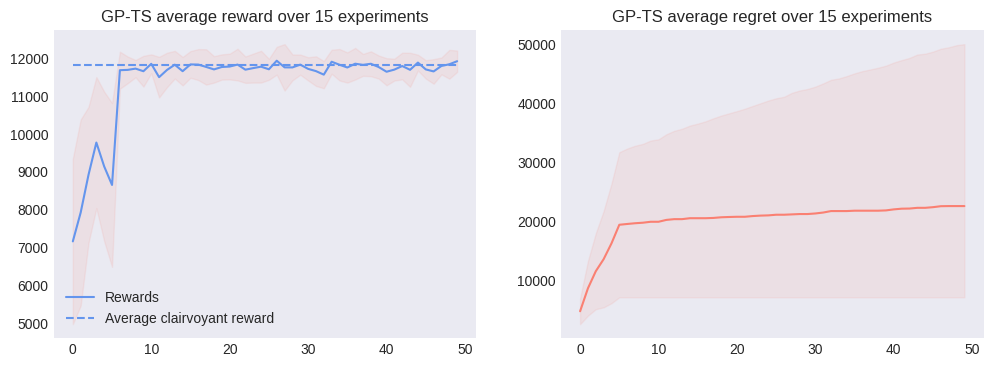
\includegraphics[scale=0.4]{img/Graphs/uncertain_alpha/image4.png}
	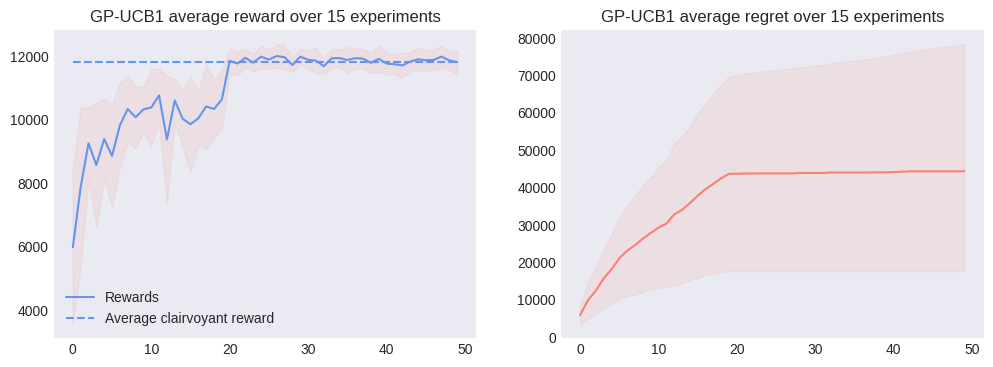
\includegraphics[scale=0.4]{img/Graphs/uncertain_alpha/image5.png}
\end{center}

\end{frame}

% ----------------------------------------

\begin{frame}[plain]

\frametitle{Average regret comparison}
\framesubtitle{Thompson Sampling and UCB}

\begin{center}
	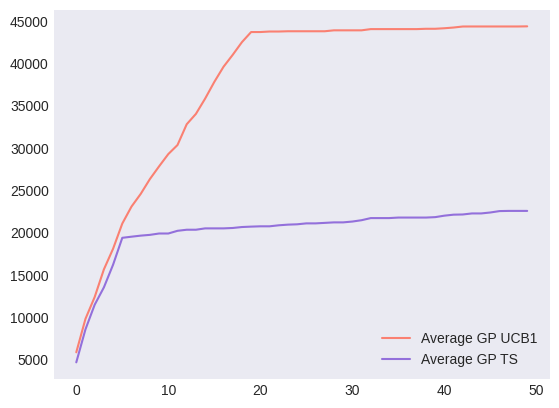
\includegraphics[scale=0.5]{img/Graphs/uncertain_alpha/image6.png}
\end{center}

\end{frame}

% ----------------------------------------

\begin{frame}

\frametitle{Results}

Overall we can observe more instability in the \textbf{TS} algorithm, but a faster convergence w.r.t to the \textbf{UCB} approach.

Both algorithms clearly converge to the optimal solution at different rates while respecting a linear cumulative regret bound.

Average results over 15 runs at time horizon $T = 50$:

\begin{table}
	\begin{tabular}{|c|cc|c|}
	\hline \hline
		\cellcolor{blue!25} & Reward 	& Regret	& Deviation \\
	\cline{2-4}
		\cellcolor{blue!25} & $\mu$		& $\mu$		& $\sigma$	\\
	\hline \hline
		GPTS 				& 11610.53 	& 31024.67	& 440.36 	\\
	\hline
		GPUCB				& 11737.73	& 43686.67	& 349.47	\\
	\hline \hline
	\end{tabular}
\end{table}

\end{frame}

% ----------------------------------------


% ----------------------------------------

% Uncertain alpha functions and number of items sold ----------------------

\section{Uncertain $\alpha$-functions and number of items sold}

% ----------------------------------------

% ----------------------------------------

\subsection{Contextual hypotesis}

% ----------------------------------------

\begin{frame}

\frametitle{Scenario}

In this case the e-commerce website doesn't register neither the \textbf{units sold} for each product nor the \textbf{class parameters}.

\todo{expand}

\end{frame}

% ----------------------------------------

\subsection{Algorithm}

% ----------------------------------------

\begin{frame}

\frametitle{Algorithm}
\framesubtitle{Algorithm outline}

so in order to work it estimate the list of values, corresponding to the earnings for each product given the knowledge obtained by the learner until now
We separately consider all the aggregated interactions where users landed on a certain product, then compute the reward they generated.
This way we obtain reward associated to a single campaign.

\todo{expand and correct}

\end{frame}

% ----------------------------------------

\subsection{Results}

% ----------------------------------------

\begin{frame}

\frametitle{Results}
\framesubtitle{}

\todo{results}

\end{frame}

% ----------------------------------------


% ----------------------------------------

% Uncertain graph weights -------------------------------------------------

\section{Uncertain Graph Weights}

% ----------------------------------------

% ----------------------------------------

\subsection{Problem}

% ----------------------------------------

\begin{frame}

\frametitle{Scenario}
\framesubtitle{Hypotesis}

In this scenario the only uncertain parameters are the \textbf{graph weights}.

Alongside the other operations, the learner will run a \textbf{graph estimation} algorithm to build an accurate representation of the graph at each time step.

Meanwhile, since the \textbf{$\alpha$-functions} are known, there is no need to estimate them and they can be applied directly in the optimization problem.

\end{frame}

% ----------------------------------------

\subsection{Implementation}

% ----------------------------------------

\begin{frame}

\frametitle{Solving the problem}
\framesubtitle{Prediction}

Since there is no need to estimate the $\alpha$-functions, the best allocation is calculated using the \texttt{find\_optimal\_superarm} function used to obtain thebest estimation when the $\alpha$-functions are known.

The only difference is that a custom graph needs to be specified since we don't have access to the real graph weights.

\end{frame}

% ----------------------------------------

\begin{frame}

\frametitle{Graph estimation}

The learner contains a graph representation that is updated at each time step; the graph representation is not updated directly but through a function called \texttt{graph\_estimate}, which collects samples from various \textbf{beta distributions} for each graph weight deleting \textit{self-loops} and non-existent edges.

The parameters of the \textbf{beta distributions} ($\alpha$ and $\beta$) are defined for each edge of the graph and represent the effective quantities that are updated whenever the function \texttt{learn} is called on the learner.

\end{frame}

% ----------------------------------------

\begin{frame}

\frametitle{Parameters update}

Whenever we want to make the \textbf{graphless learner} learn by calling its dedicated function, the learner analyzes all of the interactions given as a parameter and looks at the path that the users traversed by comparing it with the current graph representation.

If a certain edge is taken or not by a given user, the $\alpha$ and $\beta$ parameters are updated accordingly.

When \texttt{predict} is called again, the graph representation is then generated from scratch by drawing samples from the \textbf{beta distributions} with the updated parameters.

\end{frame}

% ----------------------------------------

\subsection{Results}

% ----------------------------------------

\begin{frame}[plain]

\frametitle{Reward and regret}
\framesubtitle{Graphless}

\begin{center}
	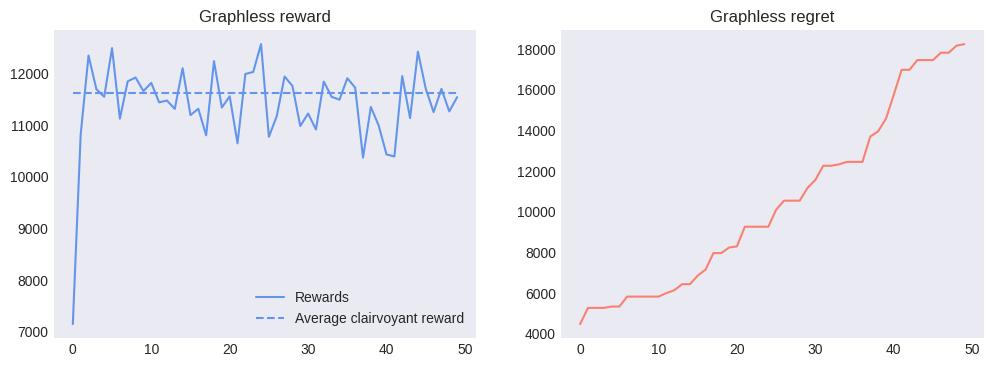
\includegraphics[scale=0.4]{img/Graphs/graphless/image1.png}
\end{center}

\end{frame}

% ----------------------------------------

\begin{frame}[plain]

\frametitle{Average reward and regret}
\framesubtitle{Graphless}

\begin{center}
	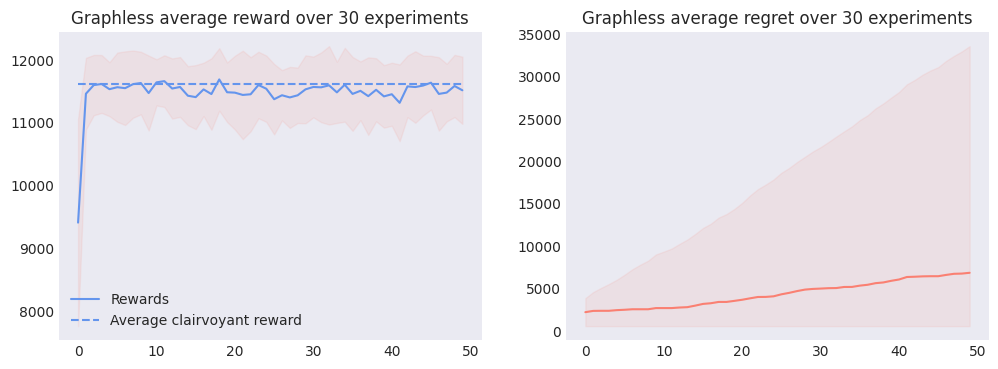
\includegraphics[scale=0.4]{img/Graphs/graphless/image2.png}
\end{center}

\vspace*{2em}

\scriptsize All tests are done using the \texttt{example\_environment} default values, \textit{population mean} of 1000, \textit{variance} of 10 and 20 \textit{budget steps}.

\end{frame}

% ----------------------------------------

\begin{frame}

\frametitle{Results}

We can observe that the regret is exceptionally low w.r.t the previous learners, this is most likely due to the fact that the \textbf{graphless learner} holds most of the important information from the environment and is able to give accurate estimations from the start.

However, some variance is always present due to the \textit{imperfect graph estimation} and \textit{environment non-determinism}.

Average results over 30 runs at time horizon $T = 50$:

\begin{table}
	\begin{tabular}{|c|cc|c|}
	\hline \hline
		\cellcolor{blue!25} & Reward 	& Regret	& Deviation \\
	\cline{2-4}
		\cellcolor{blue!25} & $\mu$		& $\mu$		& $\sigma$	\\
	\hline \hline
		Graphless			& 11515.87 	& 6845.87	& 534.97 	\\
	\hline \hline
	\end{tabular}
\end{table}

\end{frame}

% ----------------------------------------


% ----------------------------------------

% Non-stationary demand curve ---------------------------------------------

\section{Non-stationary demand curve}

% ----------------------------------------

% ----------------------------------------

\subsection{Environment behavior}

% ----------------------------------------

\begin{frame}
\frametitle{Non-stationary behavior}
\framesubtitle{Overview}

By using the \textbf{non-stationarity} assumption we are taking into consideration that the demand curve could be subject to changes over time and isn't necessarily fixed as we have seen in other steps.

There are 2 main types of \textit{non-stationary behaviors}:
\begin{itemize}[label={$\circ$}]
    \item \textbf{Abrupt changes}: where it's possible to identify different phases with different phase-wise stationary demand curves.
    \item \textbf{Smooth changes}: where the demand curve changes over time in a continuous manner.
\end{itemize}

As per specifications, we will only consider \textbf{abrupt changes} in the scope of our project.

\end{frame}

% ----------------------------------------

\begin{frame}
\frametitle{Non-stationary behavior}
\framesubtitle{Abrupt changes}

\textbf{Abrupt changes} are usually experienced when an important event strikes the market \textit{(e.g. a new product that shifts the interests of the users is released or an historical event shapes the opionion of people)}; change isn't necessarily bad, however, it may impact negatively the prediction of learners that were created with a static environment in mind.

Neither \textbf{UCB} nor \textbf{TS} account for abrupt changes since it's almost impossible for them to try a superarm that was deemed as \textit{unoptimal} over the past iterations (while it might have become optimal after an \textit{abrupt change}), therefore we expect to see a significant \textbf{reward drop} from them after an \textit{abrupt change}.

\end{frame}

% ----------------------------------------

\begin{frame}
\frametitle{Simulating abrupt changes}

In the early stages of the project we noticed that the \textbf{Simulation} that we created wasn't really fit to dinamically include abrupt changes in the environment, therefore great effort was spent in completely reworking the interface for the \textbf{Simulation} from the ground-up.

Besides collateral improvements in reproducibility, results collection and user-friendliness, the new \textbf{Simulation} allowed for an \textit{incremental simulation unfolding}, this meant that we were now able to simulate \textit{n} days, change the environment and simulate another \textit{n} days.

This particular feature revealed itself as fundamental for the upcoming challenges.

\end{frame}

% ----------------------------------------

\subsection{Algorithms}

% ----------------------------------------

\begin{frame}
\frametitle{Approaches}
\framesubtitle{Sliding window and Change detection}

There are 2 main approaches to deal with a \textbf{non-stationary environment}
\begin{itemize}[label={$\circ$}]
    \item \textbf{Sliding window}: only consider the last $\tau$ samples for predictions.
    \item \textbf{Change detection}: detect when a change has happened and adapt accordingly.
\end{itemize}

It's clear that \textbf{Sliding window} approaches are more fit for \textbf{smooth changes} while \textbf{Change detection} approaches work better with \textbf{abrupt changes}, however it's important to note that both approaches can be utilized to deal with any \textit{non-stationary} scenario.

\end{frame}

% ----------------------------------------

\begin{frame}
\frametitle{Sliding window}
\framesubtitle{Sliding window for TS and UCB}

\begin{itemize}[leftmargin=*, label={$\circ$}]
    \item \textbf{SW-GPTS} only differs in the \textbf{gaussian process} update since the older samples are progressively removed from the estimation as time goes on.
    \item \textbf{SW-GPUCB} also differs in the confidence bound formulation and the new arm choice:
        \begin{displaymath}
            a_t =
            \begin{cases}
                a_{\overline{t}} & \text{if} ~ \exists \overline{t} ~ | ~ n_{a_{\overline{t}}}(t-1, \tau) = 0 \\
                arg\max_{a \in A} \left\{ \mu_{t-1, \tau} + \delta \sigma_{t-1, \tau} \right\} & \text{otherwise}
            \end{cases}
        \end{displaymath}
\end{itemize}

\end{frame}

% ----------------------------------------

\begin{frame}
\frametitle{Change detection}

We used a \textbf{reward-based algorithm} as a \textit{change detection algorithm}, it works by comparing the last $k$ rewards with the newest $k$ rewards ($k=4$ by default) and if the difference between their means exceedes a certain threshold $\omega$ ($\omega=400$ by default) the learner is \textbf{reset} and is therefore able to learn a new optimal superarm from scratch.

Formally:
\begin{displaymath}
    \text{RESET learner if} ~ t \geq 2k ~ \land \sum_{i=t-2k}^{t-k} r_i -\sum_{i=t-k+1}^t r_i > \omega
\end{displaymath}

\scriptsize N.B. there is an offset of 1 in the representation of t between theory and code

\end{frame}

% ----------------------------------------

\subsection{Results}

% ----------------------------------------

\begin{frame}
\frametitle{}
\framesubtitle{}

\todo{insert correct image}
%\makebox[\textwidth]{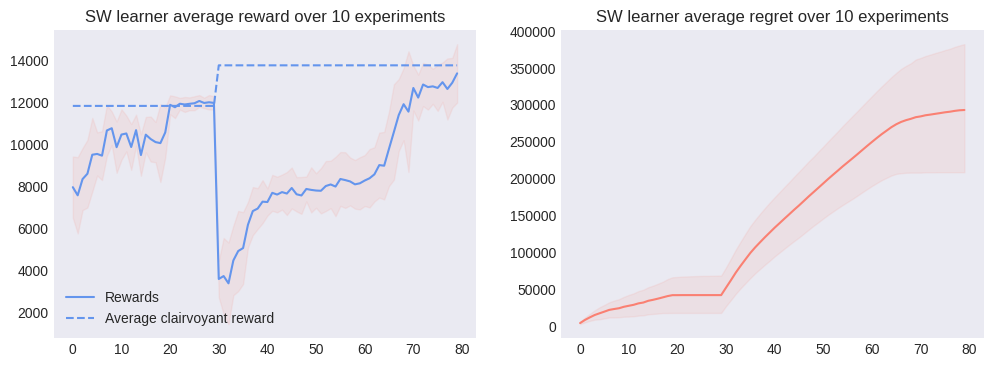
\includegraphics[width=\paperwidth]{img/Graphs/non_stationary/image2.png}}

\scriptsize Graphs representing reward and regret in the non-stationary environment with different approaches. (Only \textbf{UCB} algorithms were evaluated)

\end{frame}

% ----------------------------------------

\begin{frame}
\frametitle{Reward and regret}

We calculated the mean \textbf{reward} and \textbf{regret} considering their variance over multiple runs.

\todo{insert image}
%\makebox[\textwidth]{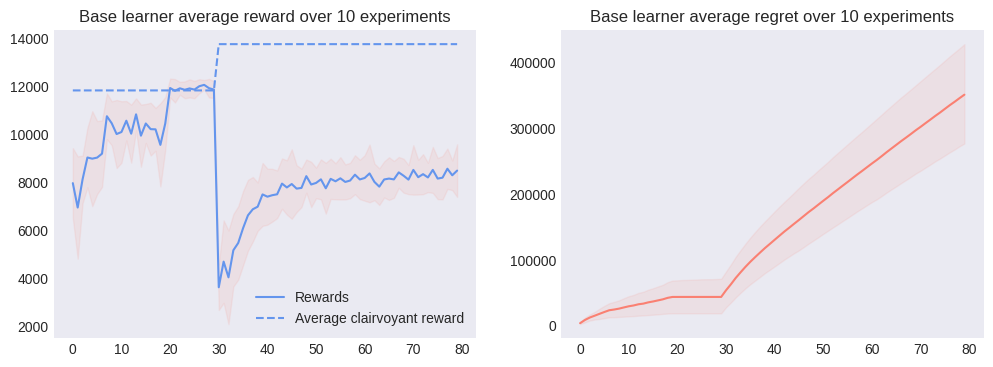
\includegraphics[width=\paperwidth]{img/Graphs/non_stationary/image1.png}}

\end{frame}

% ----------------------------------------

\begin{frame}
\frametitle{Theoretical guarantees}

In addition, if the \textbf{number of breakpoints} $m$ is small enough with respect to the \textbf{time horizon} $T$ to the power of $\alpha$ we have that the \textbf{regret} is of the order $O\left( \vert A \vert T^{\frac{1+\alpha}{2}} \right)$

\end{frame}

% ----------------------------------------


% ----------------------------------------

% Context generation -------------------------------------------------------

\section{Context generation}

% ----------------------------------------

%-----------------------------------------

\subsection{General Remarks}

%-----------------------------------------

\begin{frame}

\frametitle{Theory}
\framesubtitle{Basics}

The goal of \textbf{context generation} and \textbf{contextual bandit algorithms} is to employ a (partially) disaggregated approach in order to better exploit the differences of the users that belong to different classes.

This is made possible by using a specialized Learner for each context and an \textit{offline context generation algorithm} that decides which contexts are worth to target by isolating them from the aggregated data. This algorithm is ran every two weeks.

Each context is able to target a set of features, and a \textbf{context structure} is a set of contexts that targets all the existing features without any overlap.

\end{frame}

%-----------------------------------------

\subsection{Assumptions}

%-----------------------------------------

\begin{frame}

\frametitle{Implementation challenges}
\framesubtitle{Weaknesses}

Context generation has been, by far, the \textit{toughest} task that we faced on this whole project.

Even after many meetings and discussions we felt that there was something that didn't click with our interpretation since we didn't find a way to give a complete meaning to the dataset collected by our active bandits due to how the prediction and the rewards worked in our scenario.

In the end, our final results for this step were \textbf{unsatisfactory} and there is still wide room for improvement.

\end{frame}

%-----------------------------------------

\begin{frame}

\frametitle{Implementation assumptions}
\framesubtitle{Compromises}

Given the difficulties that we encountered, we decided to make some compromises in order to still carry out the task to an end:

\begin{itemize}[label={-}]
    \item The e-commerce website company owns a simulation capable of simulating interactions.
    \item Learners are trained on the fake simulation since we can't get enough information from the logs.
    \item The best expected reward for a given context is considered as the maximum reward experienced by a learner on a fake simulation run.
\end{itemize}

\end{frame}

%-----------------------------------------

\begin{frame}

\frametitle{Implementation assumptions}
\framesubtitle{Potential problems}

Given our interpretation, some quantities were particularly difficult to identify in a correct manner, especially the \textbf{expected value $\mu$ of the optimal arm $a^*$ for a context $c$} (written as $\mu_c$) that we resorted to calculate as the mean reward over a fake simulation on the context $c$.

Additionaly we used the \textbf{Hoeffding bound} to compute lower bounds for both the \textit{context probability} and the \textit{context expected value}.

These particular points are critical parts that absolutely need to be revisioned and most definetly are concurring causes to the unsatisfactory results.

\end{frame}

%-----------------------------------------

\subsection{Implementation}

%-----------------------------------------

\begin{frame}

\frametitle{Greedy algorithm}
\framesubtitle{Part 1 of 2}

We generate contexts following a \textbf{greedy algorithm} that, given a context $c$:

\begin{itemize}[label={*}]
    \item Considers all the possible binary 1-feature splits $\{c_i^0$, $c_i^1\}_n$ for the features not present in $c$.
    \item Creates and evaluates a new learner for each split $c_i^j$, obtaining the \textbf{context probability} $p_i^j$ and the \textbf{best expected reward} $\mu_i^j$.
    \item[] $\rightarrow$
\end{itemize}

\end{frame}

%-----------------------------------------

\begin{frame}

\frametitle{Greedy algorithm}
\framesubtitle{Part 2 of 2}

\begin{itemize}[label={*}]
    \item[] $\rightarrow$
    \item Evaluates the \textbf{splitting condition} on each couple of splits $(c_i^0$, $c_i^1)$ w.r.t the original context $c$ while deciding which split is the best one (if it exists).
    \item If a split has been made, repeat all the operations recursively on the new contexts until \textit{no split is made} or \textit{no split is possible}.
\end{itemize}

\end{frame}

%-----------------------------------------

\begin{frame}

\frametitle{Context generation}
\framesubtitle{Split condition}

Since utilizing multiple contexts is an expensive operation and our \textit{greedy algorithm} is \textbf{not} guranteed to find the optimal solution, we want to be sure that when we introuduce new contexts, it is actually worth to do so.

We use a particular \textit{splitting condition} that exploits lower bounds in order to set a higher threshold for the quality of our splits:

\begin{Large}
    \begin{displaymath}
        \underline{p}_i^0 \underline{\mu}_i^0 + \underline{p}_i^1 \underline{\mu}_i^1 \geq \underline{\mu}_i
    \end{displaymath}
\end{Large}

for context $i$ defined by a binary feature split on 0 and 1.

\end{frame}

%-----------------------------------------

\begin{frame}

\frametitle{Context utilization}

Once a certain number of contexts has been established, a \textbf{Contextual Learner} will be able to assign an \textbf{Alphaless Learner} to each context and obtain their raw predictions by utilizing the function \textbf{predict\_raw} (which returns an un-optimized array of predictions) and then running the optimization algorithm on all the predictions gathered this way.

The resulting \textit{superarm} is then passed to the \textbf{Simulation} which, in return, generates the interactions for the day by weighting the different classes according to the disaggregated predictions.

\end{frame}

%-----------------------------------------

\subsection{Results}

%-----------------------------------------

\begin{frame}

\frametitle{Results}
\framesubtitle{}

\todo{Insert results}

\end{frame}

%-----------------------------------------


% ----------------------------------------

\end{document}
